\documentclass[conference]{IEEEtran}
\usepackage{amsmath,booktabs,graphicx}
\usepackage[hidelinks]{hyperref}
\title{Solving Redactle with Article Beliefs and Masked Language Models}
\author{\IEEEauthorblockN{[Author name]}\IEEEauthorblockA{CS238, Stanford University}}
\begin{document}
\maketitle

\begin{abstract}
Redactle asks a player to recover the title of a redacted Wikipedia article by guessing one word at a time. Each guess reveals matching words and supplies evidence about the article's topic, but high-frequency words can reveal substantial text without advancing the title. We compare a belief-based agent that updates a distribution over training articles, a variant that also scores guesses with DistilRoBERTa, and a reinforcement learning policy that chooses among belief-generated candidates. On 647 held-out puzzles, the masked-language-model agent solves 87.2\% within 500 guesses, compared with 81.9\% for belief alone and 81.1\% for the learned policy. The language model also reduces mean guess cost from 186.1 to 156.5 when failures count as 500 guesses. On validation puzzles, periodically prioritizing rare words shared by related articles improves the belief agent's ability to recover the title. The results distinguish two demands of the game: identifying the topic and finding the specific words that name it.
\end{abstract}

\section{Introduction}
In Redactle, the player begins with the punctuation, common words, and hidden-word lengths of a Wikipedia article \cite{redactle}. A guess can reveal dozens of occurrences, one title word, or nothing. For example, a guess like \emph{orbital} can provide evidence about the topic of a planet article, whereas \emph{Neptune} can finish the puzzle immediately. Both actions cost one turn. The goal is to reveal every hidden title word within a fixed number of guesses.

The problem is an instance of sequential decision-making under partial observability. An agent can use a guess to gather evidence about the topic, to reveal local language that makes later guesses easier, or to attempt a title word directly. The action space is open at the environment level, and an effective policy must rank a large number of superficially plausible guesses. The title is unknown and the evaluation article is held out from the training corpus, so the agent must transfer evidence from related documents.

We ask whether word-match feedback supports useful topic inference on held-out articles, whether a masked language model improves choices beyond corpus statistics, and whether a learned candidate policy improves on a hand-designed rule. We build a controllable Redactle benchmark from Wikipedia Vital Articles and evaluate five agents on the same puzzles. The belief agent estimates thematic similarity from guess counts and periodically searches for rare words in nearby articles. The language model uses the visible context around hidden words as a second signal. The learned policy uses the same belief representation and candidate scores to decide which kind of guess to make.

\section{Related Work}
Partially observable Markov decision processes provide a framework for using observations to track hidden state and choose actions \cite{pomdp}. An exact belief for this game would require a model of possible unseen articles and the exact observation induced by a guess. We instead maintain a distribution over proxies drawn from the training corpus, using a count likelihood that can assign nonzero probability to observations absent from a given proxy. This is an approximate filter followed by a scoring rule.

Document-frequency weighting has a long history in information retrieval \cite{salton}. In our setting, an estimated occurrence count rewards words that could reveal a large amount of text. Inverse document frequency serves a different purpose. Among articles that are already judged relevant, it emphasizes words specific enough to help identify the missing title. This makes it possible to separate the scores used during topic discovery and title search.

Masked language modeling supplies context-sensitive predictions for hidden tokens. RoBERTa revisits the pretraining choices underlying masked language modeling \cite{roberta}. We use the pretrained DistilRoBERTa checkpoint \cite{distil} to predict individual hidden words with lengths compatible with the title. Proximal policy optimization (PPO) provides a way to optimize decisions over multiple steps \cite{ppo}. We use it to learn a policy over a small candidate set with generalized advantage estimation \cite{gae}. The comparison measures whether learning to select among those candidates is more effective than applying a fixed scoring rule.

\section{Environment and Data}

\subsection{Game and objective}
The hidden state consists of the article and the set of token positions already visible. The initial observation contains the article's redacted title and body. Punctuation, whitespace, and a fixed list of common words are visible. Hidden words expose their character lengths. After each guess, the observation includes the updated text, match count, and guess history. Matching removes case, accents, and apostrophes, handles possessives and pronoun families, and lemmatizes with Simplemma. One valid guess reveals all hidden tokens with its match key across the title and body. A first guess with zero matches is valid and supplies evidence. Repeated or otherwise invalid guesses count against the evaluation budget.

An episode ends when every distinct hidden title key is revealed or the agent makes 500 counted guesses. The simulator gives a reward of $-1$ per counted guess and a bonus of $500$ on success. Let $T$ be guesses to solution, with $T=\infty$ for an unsolved puzzle. We measure success at budget $b$ by $\Pr(T\leq b)$ and mean capped cost by the empirical mean of $\min(T,500)$. The capped mean includes every puzzle. The median among solved episodes describes the speed of successful runs and can move as the set of solved puzzles changes.

\subsection{Dataset construction}
We match the repository's list of 10,013 Wikipedia Vital Article titles across levels 1--4 against the English Wikipedia snapshot \texttt{20231101.en} \cite{wiki,vital}. The cached match file contains 6,575 rows. We remove final parenthetical qualifiers from titles and trim the body from the first recognized trailing heading, such as References or External links. We exclude lists and pages flagged as disambiguation, articles shorter than 300 word tokens, and pages that fail the Latin-script and prose filters. At least 95\% of alphabetic characters in both title and body must be Latin. The body must have at least 20\% tokens from the script's English stopword list. Kept titles have one to four distinct hidden match keys and at most 40 characters.

The resulting 6,472 puzzles are shuffled with Python's seed 42. The first 647 are assigned to test, the next 647 to validation, and the remaining 5,178 to training. Training-only counts include hidden word positions in titles and bodies. The vocabulary retains keys appearing in at least two training documents, leaving 128,193 keys, each represented by its most common lowercase surface form. Ties in the frequency baseline are broken by corpus token count and then by key.

\section{Agents}

\subsection{Nonadaptive baselines}
The random agent draws a uniform permutation of the vocabulary for each episode. The frequency agent visits the vocabulary in descending training document frequency. Neither changes its ranking in response to match counts or title lengths. These baselines quantify how well a fixed vocabulary order works under the same budget.

\subsection{Belief over training articles}
Let $c_{iw}$ be the count of key $w$ in training article $i$, $L_i=\sum_w c_{iw}$, and $V$ the size of the vocabulary. We define an add-one corpus background $q_w=(1+\sum_i c_{iw})/(V+\sum_i L_i)$. The initial number of hidden title and body words, $L$, is observable. The expected number of matches under proxy $i$ is
\begin{equation}
 \lambda_{iw}= L\frac{c_{iw}+\alpha q_w}{L_i+\alpha},
 \qquad \alpha=20.
\end{equation}
Starting with uniform weights, the agent updates the log weight $\ell_i$ after each valid in-vocabulary guess $w$ with observed count $y$:
\begin{equation}
 \ell_i \gets \ell_i+\tau(y\log\lambda_{iw}-\lambda_{iw}),
 \qquad \tau=0.5.
\end{equation}
The omitted $\log(y!)$ term is common to all proxies. The likelihood is tempered to reduce the influence of any one count under the simplified model. A zero-hit guess penalizes proxies that predict many hits. Updates apply to all proxies, with the largest log weight subtracted for numerical stability. For scoring, we normalize the 300 highest-weight proxies and compute $E_w=\sum_i p_i\lambda_{iw}$ over those proxies.

The ordinary score starts at $E_w$. The agent prioritizes words whose representative surface lengths occur among hidden tokens, masks previously guessed keys and mixed alphanumeric keys, and multiplies scores by 3 for lengths still hidden in the title. The title multiplier rises to 11 when the maximum normalized proxy weight reaches 0.5. Because matching merges word forms, the surface-length constraint is a heuristic. An eligible inflected occurrence can have a different length from its vocabulary representative.

\subsection{Title hunting}
A concentrated belief can track the right topic but assign little expected count to the particular word needed in the title. For example, a closely related article may mention that word once, while many other words have larger counts. We score title-length words by their presence among the 50 highest-ranked training articles, weighted by inverse rank and inverse document frequency. With $i_r$ the proxy at rank $r$, $N$ the number of training articles, and $d_w$ the document frequency, the score is
\begin{equation}
 H_w=\log(N/d_w)
 \frac{\sum_{r=1}^{50}\mathbf{1}[c_{i_r w}>0]/r}
 {\sum_{r=1}^{50}1/r}.
\end{equation}
After the concentration threshold of 0.5 is reached, the agent attempts a title hunt when at least three actions have elapsed since the previous hunt. The rank weights preserve a contribution from several related articles even if the normalized belief is nearly concentrated on a single proxy. Between hunts the agent uses the ordinary score.

\subsection{Masked language model}
The language model reads the first 300 body words, with all hidden words replaced by mask tokens. The tokenizer truncates this input to 512 subword tokens. At each retained mask whose hidden length matches a still-hidden title length, we take the model probability for each alphabetic, space-prefixed token of the same length. This restricts proposals to words the model can represent with one such token. We sum the probabilities by match key over the selected positions and scale by the initial hidden-token count divided by the number of retained masks, including masks of other lengths. This is a score extrapolated from the leading body window. The scoring assumption can be weak when the opening has a different word distribution from the rest of the article.

On ordinary turns, the language-model agent adds three times the contextual score to the belief expected count before applying the usual title-length multiplier. It can also guess keys outside the training vocabulary if their contextual score wins. Such proposals have zero corpus contribution, use the standard title multiplier of 3 even after the confidence threshold, and supply no count update to the corpus belief. Hunt turns use only the corpus-based hunt rule. The checkpoint is used as released, without task-specific language model training.

\subsection{Candidate-set reinforcement learning}
The PPO policy ranks up to 32 deduplicated candidates per turn. The hunt-enabled featurizer takes up to 13 high expected-count candidates, fills the ordinary pool toward 26 with title-length candidates, and adds up to six hunt candidates. Each candidate has 14 features, including expected matches, posterior presence, title- and body-length compatibility, corpus frequency and likelihood-ratio features, and hunt score and source. The 11 global features describe remaining redaction, belief concentration and entropy, episode progress, and recent guess feedback. The actor scores each feature vector concatenated with the global features using a shared two-layer tanh MLP with width 128. The critic receives the global features and the mean and max of the candidate features across the set, excluding padding.

We initialize the actor by behavior cloning from a candidate-restricted version of the belief rule. The teacher uses the same concentration threshold and bonuses, and hunts when neither of the preceding two guesses was marked as its best hunt word. We collect 128 teacher episodes and train for 10 epochs with minibatches of 256. In teacher and PPO training episodes, a sampled article's own row is excluded from the belief so that the agent must use other documents as proxies. The vocabulary and background rates are shared across all training episodes.

PPO runs for 200 iterations of 32 sampled training episodes each. It uses Adam at $3\times 10^{-4}$, four update epochs per iteration, minibatches of 1,024, clipping at 0.2, value loss coefficient 0.5, entropy coefficient 0.01, and gradient norm clipping at 0.5. We scale rewards by 0.01 and compute generalized advantages with $\gamma=0.999$ and $\lambda=0.95$. The run uses seed 0 and six rollout workers. Greedy validation on the first 100 validation puzzles is performed every ten iterations. The saved PPO checkpoint is the first post-initialization checkpoint attaining the highest solve rate. The frozen policy chooses its highest-scoring candidate at test time.

\section{Experimental Protocol}
All five agents play the same 647 test puzzles with a 500-guess cap. We report solve rates at 50, 100, 200, and 500 guesses, capped mean cost, and the median among solved puzzles. Runs use evaluator seed 0. The validation evaluation includes ablations of the title bonus and hunt schedule, and compares the cloned candidate policy with the selected PPO checkpoint. These variants guide configuration choice. The test results compare the final selected agents.

\paragraph{Reproduction}
From the repository root, install \texttt{requirements.txt} and run \verb|python -m scripts.data| to build the puzzles. Reuse the original \texttt{data/articles.jsonl} to recover the exact splits. When rebuilding, keep the original \texttt{data/vital\_raw.jsonl} row order. In a fresh download, parquet jobs append rows in completion order, so the same seed can produce different splits. Build the vocabulary and counts on first evaluation, or use caches from the same dataset. The repository declares dependency lower bounds, so a fresh environment can resolve different library versions.

Train the candidate policy with \verb|python -m scripts.train_ppo| and arguments \verb|--use-hunt --out checkpoints/ppo_hunt|. The exact reported evaluation uses the original \texttt{best.pt} if available. Parallel rollout completion order can affect a retraining run. Use \verb|bash scripts/run_test.sh| to evaluate all five test configurations. The script requests a hunt every three turns for the belief and language-model agents, a belief threshold of 0.5, and the hunt-enabled PPO checkpoint. It uses the default language-model weight of 3 and model \texttt{distilroberta-base}. The individual CSVs in \texttt{results/} support recalculating all test metrics without retraining or running inference.

\section{Results}

\begin{table*}[t]
\centering
\caption{Held-out test results on 647 identical puzzles. The denominator of each solve rate is 647. The capped mean includes failures at 500 guesses.}
\label{tab:test}
\begin{tabular}{lrrrrrrr}
\toprule
Agent & $\leq 50$ (\%) & $\leq 100$ (\%) & $\leq 200$ (\%) & $\leq 500$ (\%) & Solved & Capped mean & Solved median \\
\midrule
Random & 0.0 & 0.0 & 0.0 & 0.0 & 0 & 500.0 & -- \\
Frequency & 0.0 & 0.0 & 0.3 & 2.2 & 14 & 496.4 & 326 \\
Belief + hunt & 28.7 & 48.7 & 67.1 & 81.9 & 530 & 186.1 & 80.5 \\
PPO with hunt candidates & 25.3 & 45.1 & 64.0 & 81.1 & 525 & 195.6 & 83 \\
Belief + hunt + masked LM & \textbf{34.9} & \textbf{57.2} & \textbf{73.3} & \textbf{87.2} & \textbf{564} & \textbf{156.5} & \textbf{65} \\
\bottomrule
\end{tabular}
\end{table*}

\begin{figure}[t]
\centering
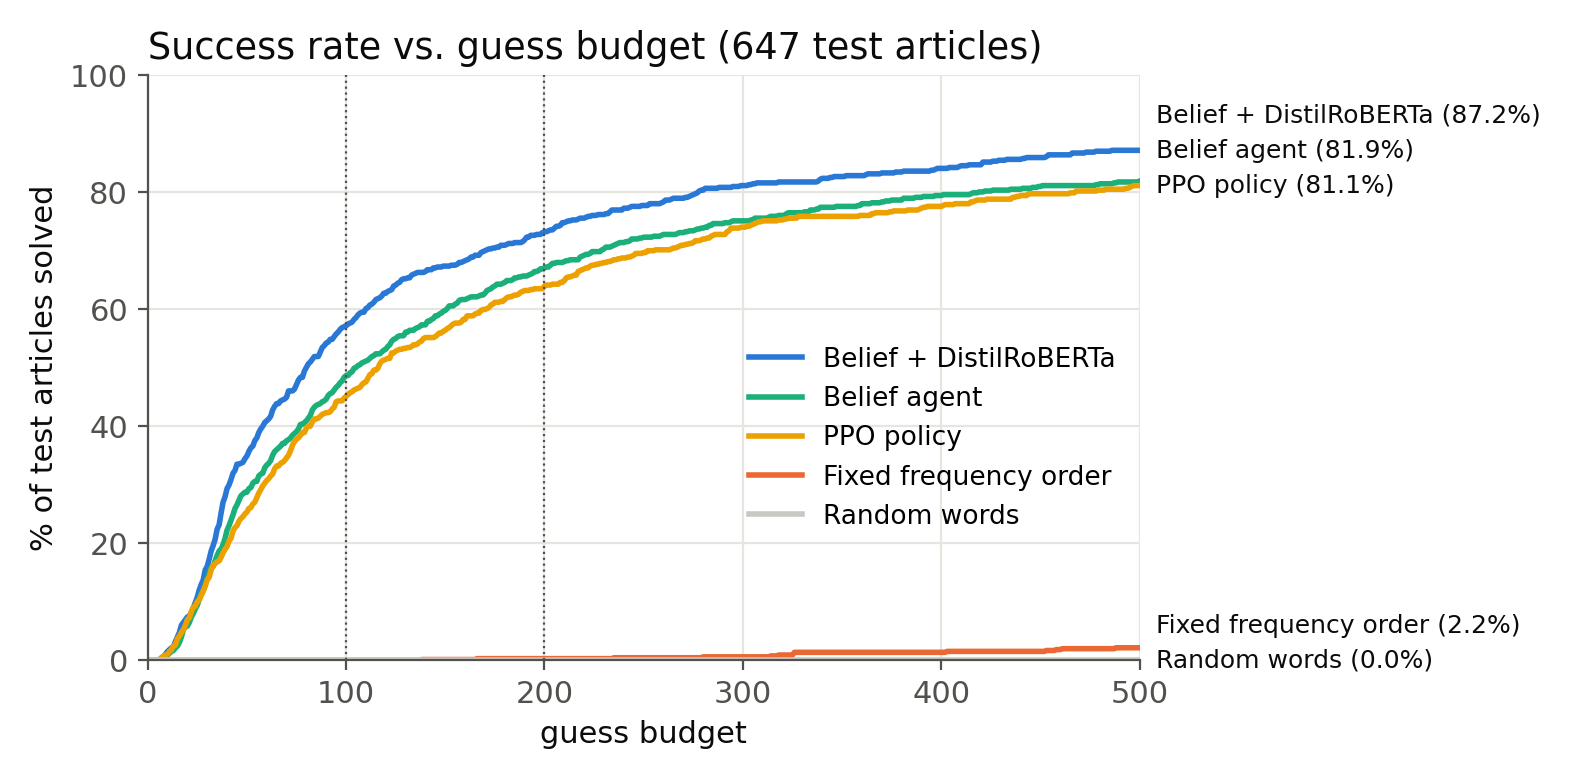
\includegraphics[width=\columnwidth]{../figures/success_vs_budget.png}
\caption{Fraction of test puzzles solved by each guess budget. The masked language model improves the solve rate at all four reported budgets.}
\label{fig:budget}
\end{figure}

\subsection{Held-out performance}
Table~\ref{tab:test} and Fig.~\ref{fig:budget} show that belief-driven agents solve substantially more puzzles than the fixed-order baselines. At 100 guesses, the language-model agent solves 370 puzzles, compared with 315 for the belief agent and 292 for PPO. At 500 guesses the language model solves 39 puzzles missed by belief alone and misses five that belief solves. This is a net gain of 34 puzzles, or 5.3 percentage points. The paired difference in capped cost is 29.5 guesses per puzzle, a 15.9\% reduction relative to belief. A paired percentile bootstrap with 3,000 resamples of the 647 puzzles and Python seed 0 gives 95\% intervals of [3.4, 7.3] percentage points for the solve-rate gain and [22.4, 37.1] guesses for the cost reduction. These intervals resample puzzle rows and describe variation across puzzles for the saved agents.

Inference time differs across agents. The logged evaluation loop took 3,550 seconds for the language-model agent, 547 seconds for belief alone, and 1,118 seconds for PPO. These times describe the recorded run and exclude agent construction. They illustrate the additional computation accompanying the language-model agent's lower guess cost.

\subsection{Validation ablations}
\begin{table}[t]
\centering
\caption{Validation results on all 647 validation puzzles.}
\label{tab:val}
\begin{tabular}{lrr}
\toprule
Configuration & Solved (\%) & Capped mean \\
\midrule
Belief, standard title bonus & 65.2 & 254.1 \\
Belief, confidence-based bonus & 69.6 & 231.3 \\
Belief, confidence bonus and hunting & 76.7 & 198.3 \\
Belief + hunt + masked LM & 81.0 & 172.5 \\
Candidate policy, behavior cloning & 68.8 & 241.4 \\
Candidate policy, after PPO & 76.8 & 210.1 \\
\bottomrule
\end{tabular}
\end{table}

Table~\ref{tab:val} shows that increasing the title bonus after the belief concentrates helps, and periodically searching by the rank-weighted rarity score produces a further gain. Adding hunts to the confidence-based bonus raises solves from 450 to 496 and reduces capped cost by 33.0 guesses. In the first-100 validation sweep, language-model weights 0.3, 1, 3, and 10 with the confidence bonus and without hunts yield solve rates of 79\%, 78\%, 79\%, and 76\%. Weight 3 has the lowest capped cost among those four runs. After adding hunts it reaches 86\% on that subset. The sweep narrows down workable settings, and small differences on 100 puzzles should be interpreted with care.

PPO improves upon behavior cloning from 445 to 497 validation solves and reduces capped cost by 31.2 guesses. The selected checkpoint is iteration 40, which reaches 83\% on the first 100 validation puzzles. On test, the learned policy solves five fewer puzzles than the belief heuristic and uses 9.6 more capped guesses on average. Its validation improvement therefore establishes that policy optimization helps this initialization. The comparison against belief also reflects differences in access to candidates. The learned policy has a short list, whereas the heuristic ranks the full eligible vocabulary.

\subsection{Illustrative episode}
In the saved validation trace for \emph{Neptune}, the title begins as one hidden seven-character word. The language-model agent eventually guesses \emph{orbital} and solves on guess 10. The corpus-only belief agent solves on guess 15. This trace illustrates how a clue can support title search and how an agent can finish with much of the body still hidden. The aggregate results quantify how often the gains extend beyond an individual puzzle.

\section{Discussion}
The fixed-order baselines have almost the entire vocabulary available yet rarely finish a puzzle. The evaluator finds that 98.8\% of test titles have all their keys in the training vocabulary. That diagnostic counts vocabulary membership alone. Length filtering, matching normalized forms, and candidate truncation can narrow the guesses available in practice. The gap between membership and observed accuracy indicates that prioritizing the right available words within the budget is an important part of the task.

The corpus and contextual models address different parts of that ranking problem. The belief update uses match counts from the whole article and can identify a topic even when the opening is heavily masked. Local context can then distinguish plausible words of the same length. The LM comparison measures the joint effect of contextual reranking and access to additional word proposals. An evaluation that holds the action vocabulary fixed would be needed to isolate those effects. Similarly, comparing PPO against the exact teacher with the same candidate list would help distinguish the effects of ranking from limits in candidate recall. The PPO experiment uses a single training seed.

The benchmark represents curated, relatively well-documented English Wikipedia topics filtered for prose and short titles. Held-out puzzle identities establish separation from the project's article statistics. The DistilRoBERTa model card identifies OpenWebText as its training data \cite{distil}. The experiment did not measure possible overlap between that corpus and test articles. Performance on newly written articles or corpora with different title conventions remains open. The approximate count model also ignores token order, models counts independently across guesses, and can concentrate on a proxy without establishing that its title is a likely answer. The concentration threshold is a policy trigger whose calibration was outside this experiment.

\section{Conclusion}
On 647 held-out Redactle puzzles, the corpus-based belief agent with title hunting solves 81.9\% within 500 guesses. Incorporating DistilRoBERTa raises the solve rate to 87.2\% and lowers mean capped guess cost by 29.5. In validation, hunting improves the belief agent over a confidence-based title bonus alone, and PPO improves the cloned policy within its candidate set. The final PPO checkpoint trails the full-vocabulary belief heuristic on held-out guess cost. For this benchmark and these configurations, count-based topic inference, a dedicated title search rule, and masked context form the strongest tested combination.

% For a group submission, insert a section here naming each contributor and
% describing their individual contributions.
\bibliographystyle{IEEEtran}
\bibliography{references}
\end{document}
